\documentclass[12pt,letterpaper]{exam}
\usepackage[lmargin=1in,rmargin=1in,tmargin=1in,bmargin=1in]{geometry}
\usepackage{../style/exams}

\usepackage{arydshln}
\usepackage{mathtools}


% -------------------
% Course & Exam Information
% -------------------
\newcommand{\course}{MAT 108: Exam 1}
\newcommand{\term}{Fall -- 2021}
\newcommand{\examdate}{10/12/2021}
\newcommand{\timelimit}{85 Minutes}

\setbool{hideans}{false} % Student: True; Instructor: False

% -------------------
% Content
% -------------------
\begin{document}

\examtitle
\instructions{Write your name on the appropriate line on the exam cover sheet. This exam contains \numpages\ pages (including this cover page) and \numquestions\ questions. Check that you have every page of the exam. Answer the questions in the spaces provided on the question sheets. Be sure to answer every part of each question and show all your work. If you run out of room for an answer, continue on the back of the page --- being sure to indicate the problem number.} 
\scores
\bottomline
\newpage

% ---------
% Questions
% ---------
\begin{questions}

% Question 1
\newpage
\question[12] Consider the following relations below:

	\[
	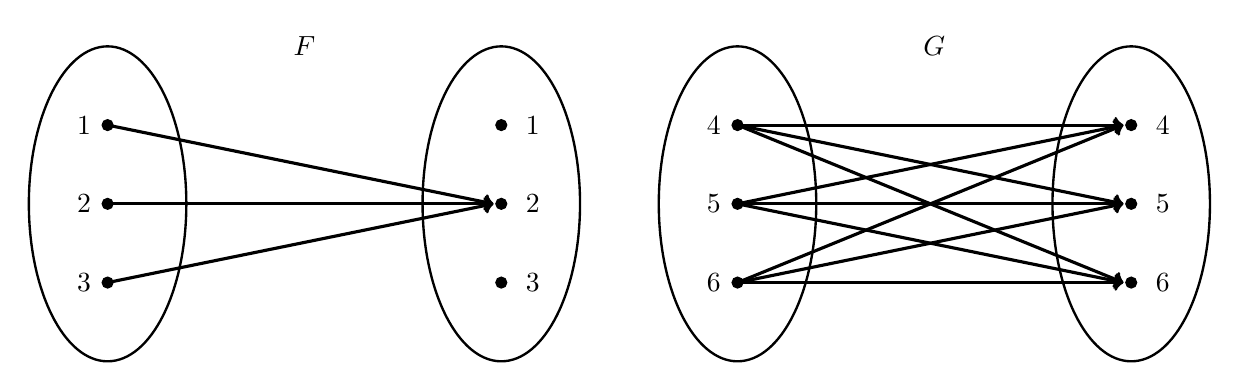
\begin{tikzpicture}
	\node at (2.5,2) {$F$};
	% Ellipses
	\draw[line width=0.03cm] (0,0) circle (1 and 2);
	\draw[line width=0.03cm] (5,0) circle (1 and 2);
	
	% Nodes
	\draw[fill=black] (0,1) circle (0.07);
	\draw[fill=black] (0,0) circle (0.07);
	\draw[fill=black] (0,-1) circle (0.07);
	
	\draw[fill=black] (5,1) circle (0.07);
	\draw[fill=black] (5,0) circle (0.07);
	\draw[fill=black] (5,-1) circle (0.07);
	
	% Arrow
	\draw[line width=0.04cm,->] (0,1) -- (4.9,0);
	\draw[line width=0.04cm,->] (0,0) -- (4.9,0);
	\draw[line width=0.04cm,->] (0,-1) -- (4.9,0);
	
	% Labels
	\node at (-0.3,1) {$1$};
	\node at (-0.3,0) {$2$};
	\node at (-0.3,-1) {$3$};
	
	\node at (5.4,1) {$1$};
	\node at (5.4,0) {$2$};
	\node at (5.4,-1) {$3$};
	
	\tikzset{shift={(8,0)}}
	%
	\node at (2.5,2) {$G$};
	% Ellipses
	\draw[line width=0.03cm] (0,0) circle (1 and 2);
	\draw[line width=0.03cm] (5,0) circle (1 and 2);
	
	% Nodes
	\draw[fill=black] (0,1) circle (0.07);
	\draw[fill=black] (0,0) circle (0.07);
	\draw[fill=black] (0,-1) circle (0.07);
	
	\draw[fill=black] (5,1) circle (0.07);
	\draw[fill=black] (5,0) circle (0.07);
	\draw[fill=black] (5,-1) circle (0.07);
	
	% Arrow
	\draw[line width=0.04cm,->] (0,1) -- (4.9,1);
	\draw[line width=0.04cm,->] (0,1) -- (4.9,0);
	\draw[line width=0.04cm,->] (0,1) -- (4.9,-1);
	\draw[line width=0.04cm,->] (0,0) -- (4.9,1);
	\draw[line width=0.04cm,->] (0,0) -- (4.9,0);
	\draw[line width=0.04cm,->] (0,0) -- (4.9,-1);
	\draw[line width=0.04cm,->] (0,-1) -- (4.9,1);
	\draw[line width=0.04cm,->] (0,-1) -- (4.9,0);
	\draw[line width=0.04cm,->] (0,-1) -- (4.9,-1);
	
	% Labels
	\node at (-0.3,1) {$4$};
	\node at (-0.3,0) {$5$};
	\node at (-0.3,-1) {$6$};
	
	\node at (5.4,1) {$4$};
	\node at (5.4,0) {$5$};
	\node at (5.4,-1) {$6$};
	\end{tikzpicture}
	\] \pspace

	\begin{minipage}[b]{0.49\textwidth}
	\centering
	\begin{tabular}{c|rcc|r}
	$x$ & $H(x)$ & \hspace{1cm} & $x$ & $J(x)$ \\ \cline{1-2} \cline{4-5}
	$1$ & $-1$ & & $5$ & $0$ \\
	$2$ & $2$ & & $6$ & $0$ \\
	$3$ & $3$ & & $8$ & $1$ \\
	$4$ & $-4$ & & $9$ & $0$ \\
	$5$ & $6$ & & $5$ & $1$
	\end{tabular}
	\end{minipage}
	\begin{minipage}[b]{0.49\textwidth}
	\[
	\begin{aligned}
	K(x)&:= 18.87x - 24 \\[0.6cm]
	L(x)&:= 2x(1 - x^8)
	\end{aligned}
	\]
	\end{minipage} \pvspace{0.6cm}
	
Determine if each of the relations given above is a function. If the relation is a function, write `T' (True) and if the relation is \emph{not} a function, write `F' (False): \pspace

	\begin{enumerate}[(a)]
	\item \usol{0.65cm}{\itshape T}: $F(x)$ \pvspace{0.3cm}
	\item \usol{0.66cm}{\itshape F}: $G(x)$ \pvspace{0.3cm}
	\item \usol{0.65cm}{\itshape T}: $H(x)$ \pvspace{0.3cm}
	\item \usol{0.66cm}{\itshape F}: $J(x)$ \pvspace{0.3cm}
	\item \usol{0.65cm}{\itshape T}: $K(x)$ \pvspace{0.3cm}
	\item \usol{0.65cm}{\itshape T}: $L(x)$
	\end{enumerate}





% Question 2
\newpage
\question[10] As accurately as possible, plot the solution set to the system of inequalities
	\[
	\begin{aligned}
	\frac{1}{3}\,x + 1&\geq y  \\
	12x + 2y &\leq 3 
	\end{aligned}
	\] \pspace

{\itshape For the first inequality, we need to plot the line $y= \frac{1}{3} x + 1$. [This is a line with slope $\frac{1}{3}$ $y$-intercept $(0,1)$.]  Because $y \leq \frac{1}{3}x + 1$, we shade beneath the line. For the second inequality, we need to plot the line $y= \frac{3}{2} - 6x$. [This is a line with slope $-6$ and $y$-intercept $(0, \frac{3}{2})$.] Because $y \leq \frac{3}{2} - 6x$, we shade beneath the line. The common region, labeled $\mathcal{R}$, is shaded below.}
	\vfill
	\[
	\begin{tikzpicture}[scale=2.2,every node/.style={scale=0.4}]
	\begin{axis}[
	grid=both,
	axis lines=middle,
	ticklabel style={fill=blue!5!white},
	xmin= -10, xmax=10,
	ymin= -10, ymax=10,
	xtick={-10,-8,...,10},
	ytick={-10,-8,...,10},
	minor tick = {-10,-9,...,10},
	xlabel=\(x\),ylabel=\(y\),
	]
	\addplot[thick, domain= -10:10] {1/3*x + 1};
	\addplot[thick, domain= -10:10] {3/2 - 6*x};
	
	\draw[draw=none,pattern=north west lines, pattern color=blue!40,opacity=0.6] (-10,10) -- (-17/12,10) -- (23/12,-10) -- (-10,-10) -- (-10,10) -- cycle;
	\draw[draw=none,pattern=north east lines, pattern color=red!40,opacity=0.6] (-10,-10) -- (-10,-7/3) -- (10,13/3) -- (10,-10) -- (-10,-10) -- cycle;
	\draw[draw=none,fill=gray,opacity=0.3] (-10,-7/3) -- (3/38,39/38) -- (23/12,-10) -- (-10,-10) -- (-10,-7/3) -- cycle;
	
	\node at (-4.5,-4.6) {\Large$\mathbf{\mathcal{R}}$};
	\end{axis}
	\end{tikzpicture}
	\]




% Question
\newpage
\question Consider the function given by $\ell(x)= 15x - 60$. \pspace

\begin{parts}
\part[2] Is this function linear? Explain. \pvspace{1.1cm}

{\itshape Yes, the function is linear---it is of the form $y= mx + b$.} \pvspace{1.3cm}


\part[2] Describe the graph of the function. \pvspace{1.1cm}

{\itshape Because the function is linear, its graph is a line.} \pvspace{1.3cm}


\part[3] What is the $x$-intercept for this function? \pspace

{\itshape
	\[
	\begin{aligned}
	\ell(x)&= 0 \\
	15x - 60&= 0 \\
	15x&= 60 \\
	x= 4
	\end{aligned}
	\]
Therefore, the $x$-intercept is $(4, 0)$.
} \pvspace{2.5cm}

\part[3] What is the $y$-intercept for this function? \pvspace{1.1cm}

{\itshape We have $\ell(0)= 15(0) - 60= -60$. Therefore, the $y$-intercept is $(0, -60)$.}
\end{parts}





% Question 4
\newpage
\question A company produces widgets. The cost function associated to production is $C(x)= 5x + 120$ and the revenue function for this product is $R(x)= 10x$. \pspace

\begin{parts}
\part[2] What are the fixed costs for production? \pvspace{1.3cm}
	\[
	C(0)= 5(0) + 120= 0 + 120= \$120
	\] \pvspace{1.4cm}


\part[2] How much does each widget cost to produce? \pvspace{1.6cm}

{\itshape Because $C(x)$ is linear, the production cost is the slope, which is $\$5$.} \pvspace{1.8cm}


\part[2] How much does the company sell each widget for? \pvspace{1.6cm}

{\itshape Because $R(x)$ is linear, the sales price of each widget is $\$10$.} \pvspace{1.8cm}
 
 
\part[6] What is the breakeven point? \pvspace{1.1cm}

{\itshape The breakeven point is when $R(x)= C(x)$, i.e. when $P(x)= 0$. So we have
	\[
	\begin{aligned}
	R(x)&= C(x) \\
	10x&= 5x + 120 \\
	5x&= 120 \\
	x&= 24
	\end{aligned}
	\]
Then the breakeven point is $(24, 240)$, i.e. when $24$ widgets are sold.}
\end{parts}





% Question 5
\newpage
\question[10] The following matrix represents an augmented system in reduced row echelon form. 
	\[
	\begin{pmatrix}
	1 & 0 & 5 & 0 & 0 & 0 & 1 \\
	0 & 1 & 0 & 0 & 0 & 0 & -2 \\
	0 & 0 & 0 & 1 & -7 & 0 & -2 \\
	0 & 0 & 0 & 0 & 0 & 1 & 3 \\
	\end{pmatrix}
	\] 
Find the set of solutions to the corresponding system of equations. \pspace

{\itshape From the second row, we know that $x_2= -2$. From the last row, we know that $x_6= 3$. Examining the columns, we know that `optimally' we should choose $x_3$ and $x_5$ as free variables. Now from the first row, we know that $x_1 + 5x_3= 1$, i.e. $x_1= 1 - 5x_3$. From the third row, we know that $x_4 - 7x_5= -2$, i.e. $x_4= 7x_5 - 2$. Therefore, the solution set to the system of equations is\dots
	\[
	\begin{cases}
	x_1= 1 - 5x_3 \\
	x_2= -2 \\
	x_3= \text{free} \\
	x_4= 7x_5 - 2 \\
	x_5= \text{free} \\
	x_6= 3	
	\end{cases}
	\]
}





% Question 6
\newpage
\question Define the following matrix:
	\[
	A= \left(
	\begin{array}{rrrr}
	2 & 0 & -5 & 1 \\
	1 & 2 & 1 & 0 \\
	-1 & 0 & -1 & 2 \\
	0 & 0 & 4 & -3 \\
	\end{array} \right)
	\]

\begin{parts}
\part[6] Compute $\det A$. \pspace

{\itshape We expand along the second column:
	\[
	\begin{aligned}
	\det A&= -0 + 2 
	\left(
	\begin{array}{rrr}
	2 & -5 & 1 \\
	-1 & -1 & 2 \\
	0 & 4 & -3 
	\end{array} \right)
	- 0 + 0= 
	2 
	\left(
	\begin{array}{rrr}
	2 & -5 & 1 \\
	-1 & -1 & 2 \\
	0 & 4 & -3 
	\end{array} \right)
	\end{aligned}
	\]
For this determinant, we expand along the last row:
	\[
	\begin{aligned}
	2 
	\left(
	\begin{array}{rrr}
	2 & -5 & 1 \\
	-1 & -1 & 2 \\
	0 & 4 & -3 
	\end{array} \right)&= 
	2 \left[
	0 - 4
	\left(
	\begin{array}{rr}
	2 & 1 \\
	-1 & 2
	\end{array} \right) -
	3 \left(
	\begin{array}{rr}
	2 & -5 \\
	-1 & -1
	\end{array} \right) \right] \\[0.3cm]
	&= 2 \bigg[ -4 \bigg( 2(2) - 1(-1) \bigg) - 3 \bigg( 2(-1) - (-5)(-1) \bigg) \bigg] \\[0.3cm]
	&= 2 \bigg[ -4(4+1) - 3 (-2 - 5) \bigg] \\[0.3cm]
	&= 2 \bigg[ -4(5) - 3(-7) \bigg] \\[0.3cm]
	&= 2 ( -20 + 21) \\[0.3cm]
	&= 2(1) \\[0.3cm]
	&= 2
	\end{aligned}
	\] 
} \vfill




\part[6] Does $A^{-1}$ exist? Explain. \pvspace{1.1cm}

{\itshape Yes, $A^{-1}$ exists because $\det A= 2 \neq 0$.} \pvspace{3.3cm}
\end{parts}





% Question 7
\newpage
\question Consider the matrix equation $A\mathbf{x}= \mathbf{b}$ given by
	\[
	\begin{pmatrix}
	-6 & 8 \\
	-5 & 7
	\end{pmatrix}
	\begin{pmatrix}
	x_1 \\
	x_2 
	\end{pmatrix}=
	\begin{pmatrix}
	-2 \\
	1
	\end{pmatrix}
	\] \pspace

\begin{parts}
\part[6] Find the inverse of the matrix $A$ in the system above. \pvspace{1.1cm}

{\itshape For a $2 \times 2$ matrix $A= \begin{pmatrix} a & b \\ c & d \end{pmatrix}$, the inverse (if it exists) is given by\dots
	\[
	A^{-1}= \dfrac{1}{\det A} \begin{pmatrix} d & -b \\ -c & a \end{pmatrix}
	\]
Now we have
	\[
	\det 
	\begin{pmatrix}
	-6 & 8 \\
	-5 & 7
	\end{pmatrix}= 
	-6(7) - 8(-5)= -42 + 40= -2
	\]
But then
	\[
	\begin{pmatrix}
	-6 & 8 \\
	-5 & 7
	\end{pmatrix}^{-1}=
	\dfrac{1}{-2} 
	\begin{pmatrix}
	7 & -8 \\
	5 & -6
	\end{pmatrix}= 
	\begin{pmatrix}
	-\frac{7}{2} & 4 \\[0.15cm]
	-\frac{5}{2} & 3
	\end{pmatrix}
	\]
} \vfill


\part[6] Use $A^{-1}$ to solve the matrix equation. \pvspace{1.1cm}

{\itshape Given a matrix equation $A\mathbf{x}= \mathbf{b}$, if $A^{-1}$ exists, we have $\mathbf{x}= A^{-1}\mathbf{b}$, simply by multiplying by $A^{-1}$ on the left on both sides. But then
	\[
	\mathbf{x}= A^{-1}\mathbf{b}= 
	\begin{pmatrix}
	-\frac{7}{2} & 4 \\[0.15cm]
	-\frac{5}{2} & 3
	\end{pmatrix}
	\begin{pmatrix}
	-2 \\
	1
	\end{pmatrix}=
	\begin{pmatrix}
	-\frac{7}{2} \cdot -2 + 4(1) \\
	-\frac{5}{2} \cdot -2 + 3(1)
	\end{pmatrix}= 
	\begin{pmatrix}
	7 + 4 \\
	5 + 3 
	\end{pmatrix}=
	\begin{pmatrix}
	11 \\
	8
	\end{pmatrix}
	\]
Therefore, $\begin{pmatrix} x_1 \\ x_2 \end{pmatrix}= \begin{pmatrix} 11 \\ 8 \end{pmatrix}$, i.e. $x_1= 11$ and $x_2= 8$. 
} \vspace{1.7cm}
\end{parts}





% Question 8
\newpage
\question[12] Compute the following:
	\[
	\begin{pmatrix}
	1 & 0 & -1 & 1 \\
	1 & 4 & 1 & 5 \\
	0 & -2 & -2 & 1 
	\end{pmatrix}
	\begin{pmatrix}
	1 & 1 \\
	2 & 2 \\
	0 & -1 \\
	1 & 0
	\end{pmatrix}
	\] \pspace

{\itshape
	\[
	\begin{aligned}
	\begin{pmatrix}
	1 & 0 & -1 & 1 \\
	1 & 4 & 1 & 5 \\
	0 & -2 & -2 & 1 
	\end{pmatrix}
	\begin{pmatrix}
	1 & 1 \\
	2 & 2 \\
	0 & -1 \\
	1 & 0
	\end{pmatrix}&= 
	\begin{pmatrix}
	1(1) + 0(2) - 1(0) + 1(1) & 1(1) + 0(2) - 1(-1) + 1(0) \\
	1(1) + 4(2) + 1(0) + 5(1) & 1(1) + 4(2) + 1(-1) + 5(0) \\
	0(1) - 2(2) - 2(0) + 1(1) & 0(1) - 2(2) - 2(-1) + 1(0) 
	\end{pmatrix} \\[0.3cm]
	&= 
	\begin{pmatrix}
	1 + 0 - 0 + 1 & 1 + 0 + 1 + 0 \\
	1 + 8 + 0 + 5 & 1 + 8 - 1 + 0 \\
	0 - 4 - 0 + 1 & 0 - 4 + 2 + 0 
	\end{pmatrix} \\[0.3cm]
	&= 
	\begin{pmatrix}
	2 & 2 \\
	14 & 8 \\
	-3 & -2
	\end{pmatrix}
	\end{aligned}
	\]
}



% Question
\newpage
\question[10] Consider the system of equations represented by the augmented matrix
	\[
	\begin{pmatrix}
	2 & 4 & 6 \\
	-1 & -5 & 3
	\end{pmatrix}
	\]
By placing the matrix in reduced row echelon form, solve the corresponding system of equations. \pspace

{\itshape
	\begin{minipage}[t]{0.49\textwidth}
	\[
	\begin{pmatrix}
	2 & 4 & 6 \\
	-1 & -5 & 3
	\end{pmatrix}
	\] \pvspace{1cm}
	\[
	\begin{pmatrix}
	1 & 2 & 3 \\
	-1 & -5 & 3
	\end{pmatrix}
	\] \pvspace{1cm}
	\[
	\begin{pmatrix}
	1 & 2 & 3 \\
	0 & -3 & 6
	\end{pmatrix}
	\] \pvspace{1cm}
	\[
	\begin{pmatrix}
	1 & 2 & 3 \\
	0 & 1 & -2
	\end{pmatrix}
	\] \pvspace{1cm}
	\[
	\begin{pmatrix}
	1 & 0 & 7 \\
	0 & 1 & -2
	\end{pmatrix}
	\]
	\end{minipage}
	\begin{minipage}[t]{0.49\textwidth} \pvspace{0.3cm}
	$\frac{1}{2} R_1 \to R_1$ \pvspace{1.8cm}
	$R_1 + R_2 \to R_2$ \pvspace{1.9cm}
	$-\frac{1}{3}R_2 \to R_2$ \pvspace{1.9cm}
	$-2R_2 + R_1 \to R_1$
	\end{minipage} \pvspace{1.1cm}
Therefore, we have $(x_1, x_2)= (7, -2)$, i.e. $x_1= 7$ and $x_2= -2$. 
	\[
	\begin{cases}
	x_1= 7 \\
	x_2= -2
	\end{cases}
	\]
}


\end{questions}
\end{document}